%%%%%%%%%%%%%%%%%%%%%%%%%%%%%%%%%%%%%%%%%
% Class Notes Template
% LaTeX Template
% By: Ryan Grove
%%%%%%%%%%%%%%%%%%%%%%%%%%%%%%%%%%%%%%%%%

%----------------------------------------------------------------------------------------
%	PACKAGES AND OTHER DOCUMENT CONFIGURATIONS
%----------------------------------------------------------------------------------------

\documentclass[paper=a4, fontsize=11pt]{scrartcl} % A4 paper and 11pt font size

\usepackage[T1]{fontenc} % Use 8-bit encoding that has 256 glyphs
\usepackage{fourier} % Use the Adobe Utopia font for the document - comment this line to return to the LaTeX default
\usepackage[english]{babel} % English language/hyphenation
\usepackage{amsmath,amsfonts,amsthm} % Math packages

\usepackage{lipsum} % Used for inserting dummy 'Lorem ipsum' text into the template

\usepackage{sectsty} % Allows customizing section commands
\allsectionsfont{\centering \normalfont\scshape} % Make all sections centered, the default font and small caps

\usepackage{fancyhdr} % Custom headers and footers
\pagestyle{fancyplain} % Makes all pages in the document conform to the custom headers and footers
\fancyhead{} % No page header - if you want one, create it in the same way as the footers below
\fancyfoot[L]{} % Empty left footer
\fancyfoot[C]{} % Empty center footer
%\fancyfoot[R]{\thepage} % Page numbering for right footer
\renewcommand{\headrulewidth}{0pt} % Remove header underlines
\renewcommand{\footrulewidth}{0pt} % Remove footer underlines
\setlength{\headheight}{13.6pt} % Customize the height of the header

\numberwithin{equation}{section} % Number equations within sections (i.e. 1.1, 1.2, 2.1, 2.2 instead of 1, 2, 3, 4)
\numberwithin{figure}{section} % Number figures within sections (i.e. 1.1, 1.2, 2.1, 2.2 instead of 1, 2, 3, 4)
\numberwithin{table}{section} % Number tables within sections (i.e. 1.1, 1.2, 2.1, 2.2 instead of 1, 2, 3, 4)

\setlength\parindent{0pt} % Removes all indentation from paragraphs - comment this line for an assignment with lots of text

\usepackage{lastpage}
\usepackage{fancyhdr}
\cfoot{\thepage\ of \pageref{LastPage}}

\def\v{\hbox{$\mathbf v$}}
\def\w{\hbox{$\mathbf w$}}
\def\u{\hbox{$\mathbf u$}}
\def\x{\hbox{$\textbf{x}$}}
\def\z{\hbox{$\mathbf z$}}
\def\a{\hbox{$\mathbf a$}}
\def\b{\hbox{$\mathbf b$}}
\def\L{\hbox{$\mathcal L$}}
\def\C{\hbox{$\mathbb C$}}
\def\B{\hbox{$\mathcal B$}}
\def\R{\hbox{$\mathbb R$}}
\def\X{\hbox{$\underline X$}}
\def\Q{\hbox{$\mathbb Q$}}
\def\R{\hbox{$\mathbb R$}}
\def\N{\hbox{$\mathbb N$}}
\def\C{\hbox{$\mathbb C$}}
\def\0{\hbox{$\mathbf 0$}}
\def\Y{\hbox{$\underline Y$}}
\def\a{\hbox{$\mathbf a$}}
\def\u{\hbox{$\mathbf u$}}
\def\w{\hbox{$\mathbf w$}}
\def\y{\hbox{$\mathbf y$}}
\def\X{\hbox{$\underline X$}}
\def\dd{\hbox{$\partial $}}
\def\B{\hbox{$\mathcal B$}}
\def\F{\hbox{$\mathcal F$}}
\def\L{\hbox{$\mathcal L$}}
\def\M{\hbox{$\mathcal M$}}
\def\D{\hbox{$\mathscr {D}$}}
\def\RR{\hbox{$\mathscr{R}$}}
\def\I{\hbox{$\mathcal I$}}

\usepackage{amssymb}
%\theoremstyle{plain}
\usepackage[margin = .75in]{geometry}
\newtheorem{claim}{Claim}
\newtheorem{theorem}{Theorem}[section]
\newtheorem{lemma}[theorem]{Lemma}
\newtheorem{proposition}[theorem]{Proposition}
\newtheorem{corollary}[theorem]{Corollary}
\newtheorem{problem}[theorem]{Problem}
%\theoremstyle{definition}
\newtheorem{definition}[theorem]{Definition}
%\theoremstyle{remark}
\newtheorem{remark}[theorem]{Remark}
\newtheorem{remarks}[theorem]{Remarks}
\newtheorem{example}[theorem]{Example}
\newcommand{\ds}{\displaystyle}
\newcommand{\ZZ}{\mathbb{Z}}
\newcommand{\QQ}{\mathbb{Q}}
\newcommand{\e}{\varepsilon}
\newcommand{\bbf}{\textbf}
\newcommand{\p}{\parallel}
\usepackage{color}
\newcommand{\field}[1]{\mathbb{#1}}
\usepackage{amsmath}
\usepackage{amsthm}
\usepackage{amssymb}
\usepackage{mathrsfs}
\usepackage{cancel}
\usepackage{upgreek}
\usepackage{graphicx}
\usepackage{multirow}
\usepackage{setspace}
\usepackage{url}
\usepackage{subfigure}
\usepackage{enumerate}
\usepackage{cases}
\usepackage{mathrsfs}
\usepackage{rotating}

%----------------------------------------------------------------------------------------
%	TITLE SECTION
%----------------------------------------------------------------------------------------

\newcommand{\horrule}[1]{\rule{\linewidth}{#1}} % Create horizontal rule command with 1 argument of height

\title{	
\normalfont \normalsize 
\textsc{Ryan Grove, Clemson University, MATH1080 - 9} \\ [25pt] % Your name, university, class
\horrule{0.5pt} \\[0.4cm] % Thin top horizontal rule
\huge Section 8.3: Moments and Center of Mass \\ % The assignment title
\horrule{2pt} \\[0.5cm] % Thick bottom horizontal rule
}

\author{Date:} % The due date

\date{\normalsize February 22, 2016} % A custom date

\begin{document}

\maketitle % Print the title

\begin{flushleft}
\begin{tabular}{l l}
Name: \rule{3.2in}{.01cm}  & {}%Table number: \rule{1in}{.01cm}\\
\end{tabular}
\end{flushleft}

%----------------------------------------------------------------------------------------
%	Lecture
%----------------------------------------------------------------------------------------

\section*{\textbf{Lecture:}}
Among the many applications of integral calculus to physics and engineering, we consider two here: force due to water pressure and centers of mass. As with previous applications to geometry ( areas, volumes, and lengths) and to work, our strategy is to break up the physical quantity into a large number of small parts, approximate each small part, sum the results, take the limit, and then evaluate the resulting integral.\\
\indent

%\section*{Hydrostatic Pressure and Force}
%
%Deep-sea divers realize that water pressure increases as they dive deeper. This is because the weight of the water above them increases.\\
%\indent
%
%In general, suppose that a thin horizontal plate with area $A$ square meters is submerged in a fluid of density $\rho$ kilograms per cubic meter at a depth $d$ meters below the surface of the fluid as in Figure 1.
%\[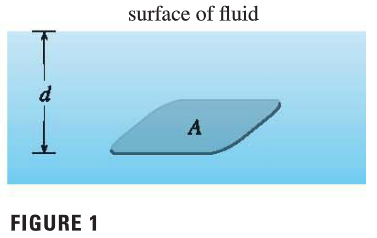
\includegraphics[scale=0.5]{8-3pic1.png}\]
%
%The fulid directly above the plate has volume \underline{\hspace{0.75in}}, so its mass is $m=\underline{\hspace{1.5in}}.$ The force exerted by the fluid on the plate is therefore
%
%\[F= \underline{\hspace{0.5in}} = \underline{\hspace{0.5in}} = \underline{\hspace{1in}}.\]
%\indent
%
%where $g$ is the acceleration due to gravity. The \textbf{pressure} $P$ on the plate is defined to be the force per unit area:
%
%\[P = \ds\frac{F}{A} = \underline{\hspace{0.75in}}.\]
%\indent
%
%The SI unit for measuring pressure is newtons per square meter, which is called a pascal (abbreviation: 1 $N/m^2 = 1 Pa$). Since this is a small unit, the kilopascal $(kPa)$ is often used. For instance, because the density of water is $\rho=1000$ $kg/m^3$, the pressure at the bottom of a swimming pool 2 meters deep is:
%
%\begin{align*}
%P &= \rho g d = \underline{\hspace{2in}\\
%&= \underline{\hspace{1.25in}} = \underline{\hspace{1.25in}}
%\end{align*}
%\indent
%
%An important principle of fluid pressure is the experimentally verified fact that \textit{at any point in a liquid the pressure is the same in all directions}. (A diver feels the same pressure on nose and both ears.) Thus the pressure in any direction at a depth $d$ in a fluid with mass density $\rho$ is given by 
%
%\[P = \rho g d = \delta d.\]
%
%This helps us determine the hydrostatic force against a \textit{vertical} plate or wall or dam in a fluid. This is not a straightforward problem because the pressure is not constant but increases as the depth increases.\\
%\indent
%
%\underline{Example 1}: 

\section*{Moments and Centers of Mass}
Our main objective here is to find the point $P$ on which a thin plate of any given shape balances horizontally as in Figure 5. The point is called the \underline{\hspace{1in}} \underline{\hspace{0.25in}} \underline{\hspace{1in}} (or center of gravity) of the plate.

\[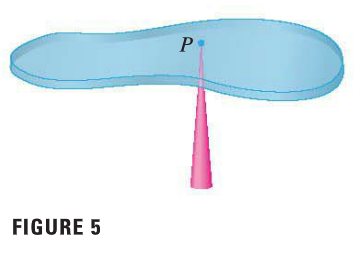
\includegraphics[scale=0.5]{8-3pic5.png}\]
\indent

We first consider the simpler situation illustrated in Figure 6, where two masses $m_1$ and $m_2$ are attached to a rod of negligible mass on opposite sides of a fulcrum and at distances $d_1$ and $d_2$ from the fulcrum. \\

\[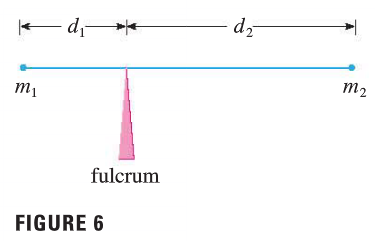
\includegraphics[scale=0.5]{8-3pic6.png}\]
\indent

 The rod will balance if

\[m_1 d_1 = m_2 d_2 \hspace{2in} (1)\]
\indent

This is an experimental fact discovered by Archimedes and called the Law of the Lever. (Think of a lighter person balancing a heavier one on a seesaw by sitting farther away from the center.)\\
\indent Now suppose that the rod lies along the $x-$axis with $m_1$ at $x_1$ and $m_2$ at $x_2$ and the center of mass at $\bar{x}$. \\

\[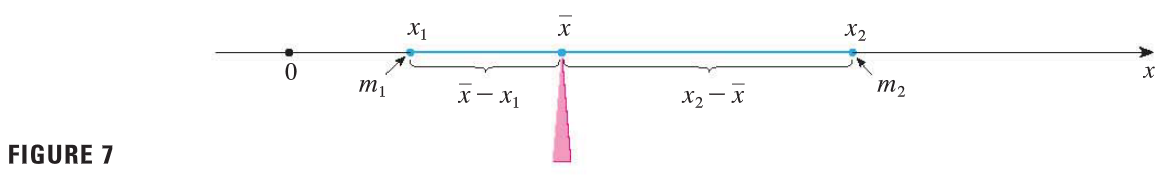
\includegraphics[scale=0.4]{8-3pic7.png}\]
\indent

 If we compare Figures 6 and 7, we see that $d_1 = \bar{x} - x_1$ and $d_2 = x_2 - \bar{x}$ and so Equation (1) gives:

\vspace{2.5in}

The numbers $m_1 x_1$ and $m_2 x_2$ are called the \underline{\hspace{1.1in}} of the masses $m_1$ and $m_2$ (with respect to the origin), and Equation $(3)$ says that the center of mass $\bar{x}$ is obtained by adding the moments of the masses and dividing by the total mass $m=m_1 + m_2$.\\
\indent

In general, if we have a system of $n$ particles with masses $m_1,m_2,\ldots,m_n$ located at the points $x_1,x_2,\ldots,x_n$ on the $x-$axis, it can be shown similarly that the center of mass of the system is located at

\[\bar{x} = \ds\frac{\ds\sum_{i=1}^n m_i x_i}{\ds\sum_{i=1}^n m_i} = \ds\frac{\ds\sum_{i=1}^n m_i x_i}{m} \hspace{2in} (4) \]

where $m=\ds\sum_{i=1}^n m_i$ is the total mass of the system, and the sum of the individual moments

\[M = \ds\sum_{i=1}^n m_i x_i\]

is called the \underline{\textbf{moment of the system about the origin}}. Then Equation 4 could be rewritten as $m\bar{x} = M$, which says that if the total mass were considered as being concentrated at the center of mass $\bar{x}$, then its moment would be the same as the moment of the system.\\
\indent

Now we consider a system of $n$ particles with masses $m_1,m_2,\ldots, m_n$ located at the points $(x_1,y_1),(x_2,y_2),\ldots,(x_n,y_n)$ in the $xy-$plane as shown here:\\
\[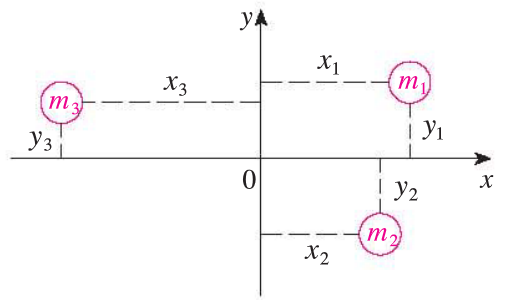
\includegraphics[scale=0.4]{8-3pic8.png}\]

By analogy with the one-dimensional case, we define the...\\
\indent

 $\bullet$ \textbf{moment of the system about the $\mathbf{y-}$axis}: \quad $M_y = \ds\sum_{i=1}^n m_i x_i$\\
 \indent

$\bullet$ \textbf{moment of the system about the $\mathbf{x-}$axis}:  \quad $M_x = \ds\sum_{i=1}^n m_i y_i.$\\
\indent

Then,\\
$\bullet$ \text{ } $M_y$ measures the tendency of the system to rotate about the $y-$axis and\\
$\bullet$ \text{ } $M_x$ measures the tendency to rotate about the $x-$axis.\\
\indent

As in the one-dimensional case, the coordinates $(\bar{x},\bar{y})$ of the center of mass are given in terms of the moments by the formulas

\[\bar{x} = \ds\frac{M_y}{m} \quad \quad \bar{y}=\ds\frac{M_x}{m}\]

where $m=\ds\sum_{i=1}^n m_i$ is the total mass.\\
\indent

\underline{Example 1}: Find the moments and center of mass of the system of objects that have masses $3,4,$ and $8$ at the points $(-1,1), (2,-1),$ and $(3,2)$, respectively.\\
\indent

SOLUTION:\\
\indent

\vspace{3in}

Next we consider a flat plate (called a \textit{lamina}) with uniform density $\rho$ that occupies a region $\mathcal{R}$ of the plane. We wish to locate the center of mass of the plate, which is called the \underline{\hspace{1.25in}} of $\mathcal{R}$. Suppose that the region $\mathcal{R}$ is of the type shown here:

\[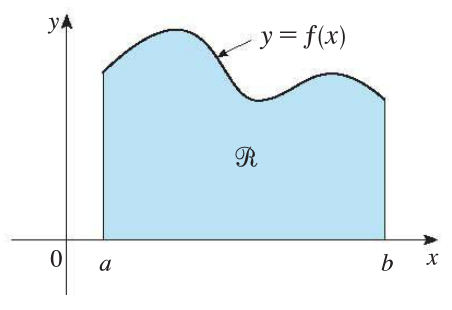
\includegraphics[scale=0.4]{8-3pic10.png}\]
\indent

that is; $\mathcal{R}$ lies between the lines $x=a$ and $x=b$, above the $x-$axis, and beneath the graph of $f$, where $f$ is a continuous function. Skipping the derivation (which can be found in section 8.3 on page 556 of the textbook), we obtain...\\

$\bullet$ The moment of $\mathcal{R}$ about the $y-$axis: \quad $\boxed{\text{ }M_y = \rho\ds\int_a^b x f(x) \text{ }dx \text{ }}$\\
\indent

$\bullet$ The moment of $\mathcal{R}$ about the $x-$axis: \quad $\boxed{\text{ }M_x = \rho\ds\int_a^b \ds\frac{1}{2}[f(x)]^2\text{ }dx \text{ }}$\\
\indent

Just as for systems of particles, the center of mass of the plate is defined so that $m\bar{x} = M_y$ and $m\bar{y} = M_x$. But the mass of the plate is the product of its density and its area:

\[m = \rho A = \underline{\hspace{1.5in}}\]

and so,\\

\begin{align*}
\bar{x} &= \ds\frac{M_y}{m} = \ds\frac{\hspace{1.5in}}{\text{ }} = \ds\frac{\hspace{1.5in}}{\text{ }}\\
\text{ }\\
\text{ }\\
\bar{y} &= \ds\frac{M_x}{m} = \ds\frac{\hspace{1.5in}}{\text{ }} = \ds\frac{\hspace{1.5in}}{\text{ }}\\
\end{align*}
\indent

Notice the cancellation of the $\rho$'s. The location of the center of mass is independent of the density. \\
\indent

In summary, the \textbf{center of mass} of the plate (or the centroid of $\mathcal{R}$) is located at the point $(\bar{x},\bar{y})$, where

\[\boxed{\text{ } \bar{x} = \ds\frac{1}{A}\ds\int_a^b x f(x)\text{ }dx \hspace{0.5in} \bar{y} = \ds\frac{1}{A}\ds\int_a^b\ds\frac{1}{2}[f(x)]^2 \text{ } dx\text{ }}\]
\indent\\

\newpage
\underline{Example 2}: Find the center of mass of a semicircular plate of radius $r$.\\
\indent

SOLUTION:\\
\indent

\newpage
\underline{Example 3}: Find the centroid of the region bounded by the curves $y=\cos x, y=0, x=0,$ and $x=\ds\frac{\pi}{2}$.\\
\indent

SOLUTION:\\
\indent

\newpage

If the region $\mathcal{R}$ lies between two curves $y=f(x)$ and $y=g(x)$, where $f(x) \geq g(x)$, then the centroid of $\mathcal{R}$ is $(\bar{x},\bar{y})$, where

\[\boxed{\text{ }\bar{x} = \ds\frac{1}{A} \ds\int_a^b x[f(x) -g(x)]\text{ }dx \hspace{0.5in} \bar{y} = \ds\frac{1}{A} \ds\int_a^b \ds\frac{1}{2}\lbrace [f(x)]^2 - [g(x)]^2\rbrace \text{ }dx \text{ }}\]
\indent

\underline{Example 4}: Find the centroid of the region bounded by the line $y=x$ and the parabola $y=x^2$.\\
\indent

SOLUTION:\\
\indent

%\fbox{
%  \parbox{\textwidth}{
%  \vspace{5pt}

















%----------------------------------------------------------------------------------------

\end{document}